\documentclass[11pt]{article}

\usepackage{sectsty}
\usepackage{graphicx}

\usepackage{listings}
\usepackage{xcolor}

\usepackage{tikz}
\usetikzlibrary{arrows.meta, quotes}
\definecolor{dkgreen}{rgb}{0,0.6,0}
\definecolor{gray}{rgb}{0.5,0.5,0.5}
\definecolor{mauve}{rgb}{0.58,0,0.82}

\renewcommand{\familydefault}{\sfdefault}
\newcommand\func[1]{\textcolor{blue}{\texttt{#1}}}

\lstdefinestyle{myScalastyle}{
  frame=tb,
  language=scala,
  aboveskip=3mm,
  belowskip=3mm,
  showstringspaces=false,
  columns=flexible,
  basicstyle={\small\ttfamily},
  numbers=none,
  numberstyle=\tiny\color{gray},
  keywordstyle=\color{blue},
  commentstyle=\color{dkgreen},
  stringstyle=\color{mauve},
  frame=single,
  breaklines=true,
  breakatwhitespace=true,
  tabsize=3,
}
% Margins
\topmargin=-0.45in
\evensidemargin=0in
\oddsidemargin=0in
\textwidth=6.5in
\textheight=9.0in
\headsep=0.25in

\title{Scala Circe}
\author{ Ramy Tanios }
\date{\today}

\begin{document}
\maketitle	
\pagebreak


\section{Summary}



    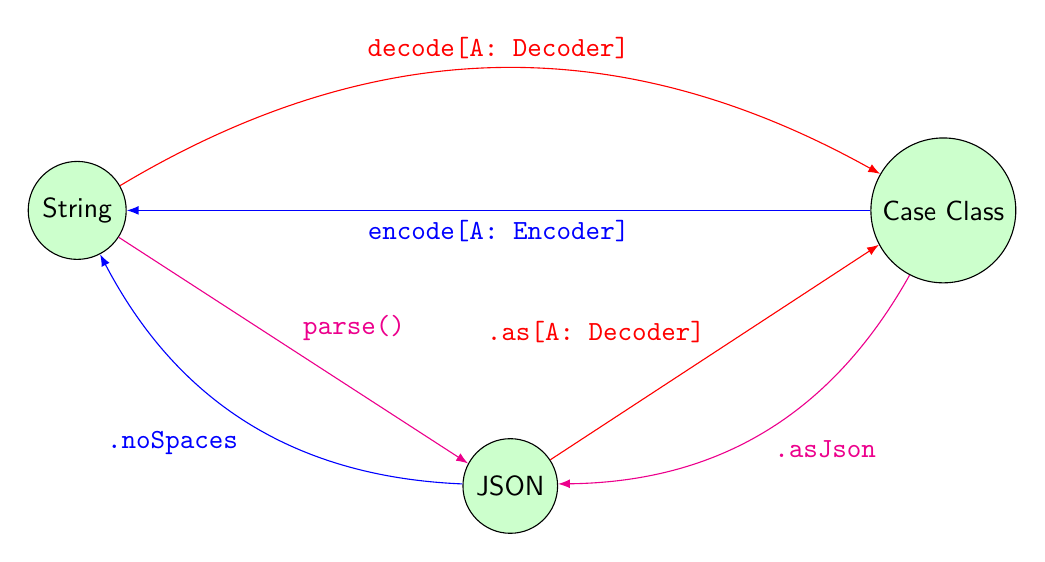
\begin{tikzpicture}[%overlay,remember picture, % do you really need this?
%
    auto,
    leaf/.style={circle,draw,fill=green!20,minimum size=1mm},
     Arr/.style={-{Latex[length=1.5mm]}},
                        ]
    \node[leaf] (json_node)  at (0,-2) {JSON};
    \node[leaf](string_node)        at (-5.5,1.5) {String};
    \node[leaf](cc_node) at (5.5, 1.5){Case Class};
    
    \draw[Arr, magenta] (string_node)   to [left=30,"\texttt{parse()}"] (json_node);
    \draw[Arr, red] (string_node)  to [bend left=30,"\texttt{decode[A: Decoder]}"]   (cc_node);
    \draw[Arr, magenta] (cc_node)  to [bend left=30,"\texttt{.asJson}"]   (json_node);
    \draw[Arr, red] (json_node)  to [left=30,"\texttt{.as[A: Decoder]}"]   (cc_node);
    \draw[Arr, blue] (json_node)  to [bend left=30,"\texttt{.noSpaces}"]   (string_node);
     \draw[Arr, blue] (cc_node)  to [left=30,"\texttt{encode[A: Encoder]}"]   (string_node);
    
    \end{tikzpicture}
    
   
\section {Contramap \& emap}
\textbf{Contramap}: Creates a new encoder that applies first a function than the old encoder.
\begin{lstlisting}[style=myScalastyle]
implicit val encodeInstant: Encoder[Instant] = Encoder.encodeString.contramap[Instant](_.toString)}
\end{lstlisting}
    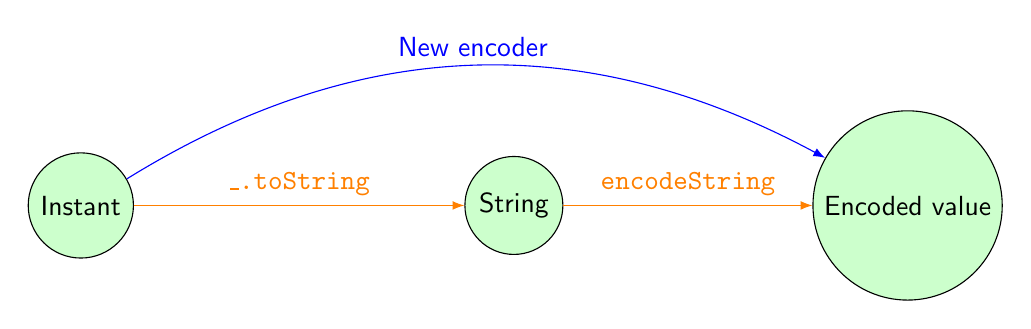
\begin{tikzpicture}[%overlay,remember picture, % do you really need this?
%
    auto,
    leaf/.style={circle,draw,fill=green!20,minimum size=1mm},
     Arr/.style={-{Latex[length=1.5mm]}},
                        ]
    \node[leaf] (instant_node)  at (-5.5,0) {Instant};
    \node[leaf](string_node)        at (0,0) {String};
    \node[leaf](encoded_node) at (5, 0){Encoded value};
    \draw[Arr, orange] (instant_node)   to [left=30,"\texttt{\_.toString}"] (string_node);
    \draw[Arr, orange] (string_node)   to [left=30,"\texttt{encodeString}"] (encoded_node);
    \draw[Arr, blue] (instant_node)   to [bend left=30,"New encoder "] (encoded_node);
    
\end{tikzpicture}

\textbf{Emap}: Creates a new decoder by applying the old decoder and then a function.
\begin{lstlisting}[style=myScalastyle]
implicit val decodeInstant: Decoder[Instant] = Decoder.decodeString.emapTry { str =>
  Try(Instant.parse(str))
}\end{lstlisting}
    \begin{tikzpicture}[%overlay,remember picture, % do you really need this?
%
    auto,
    leaf/.style={circle,draw,fill=green!20,minimum size=1mm},
     Arr/.style={-{Latex[length=1.5mm]}},
                        ]
    \node[leaf] (raw_node)  at (-5.5,0) {Raw value};
    \node[leaf](string_node)        at (0,0) {String};
    \node[leaf](instant_node) at (5, 0){Instant};
    \draw[Arr, orange] (raw_node)   to [left=30,"\texttt{decodeString}"] (string_node);
    \draw[Arr, orange] (string_node)   to [left=30,"\texttt{str => Try(\dots)}"] (encoded_node);
    \draw[Arr, blue] (raw_node)   to [bend left=30,"New decoder"] (instant_node);
    
\end{tikzpicture}


\end{document}
